\documentclass[]{article}
\usepackage{enumitem,amssymb,tikz,siunitx, pgfplots}
\usetikzlibrary{calc,matrix, arrows.meta, positioning, decorations,decorations.markings, math}
%opening
\title{Generador De Ondas Sobre Raspberry Pi Pico}
\author{Santiago Calligari, Gerónimo Nestares}
\begin{document}
\maketitle

\section*{Preámbulo}
En este artículo vamos a contar el proceso sobre la generación de ondas sinusoidales en una placa de desarrollo, vamos a exponer todos los obstáculos que nos topamos, las soluciones que les dimos y las ideas tanto matemáticas como electrónicas que utilizamos para poder hacer esta idea una realidad que pueda ser replicada.\\
Nuestra placa de desarrollo cuenta con algunos pines \textbf{G.P.I.O.} (General Purpouse Input/Output) que son utilizados para propósitos generales de entrada/salida. Nosotros vamos a utilizar uno de estos pines para llegar a nuestra onda sinusoidal, pero nos encontramos con un problema ¡No existen las ondas analógicas en el mundo digital! Nosotros contamos solamente con una función "prendido" que nos entrega 5V en nuestro pin y una función "apagado" que nos entrega 0V. Aquí entra nuestro primer concepto a explicar, la modulación por ancho de pulsos.
\section*{Modulación Por Ancho de Pulsos}
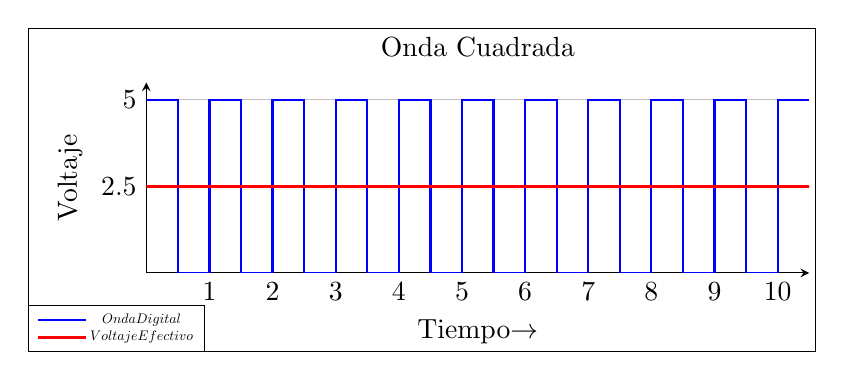
\begin{tikzpicture}
	\draw (-1.5,-1) -- (8.5,-1) -- (8.5,3.1) -- (-1.5,3.1) -- (-1.5,-1);
	\begin{axis}[
		legend style={nodes = {scale=0.5, transform shape}, at={(0.088,-0.17)}},
		legend entries={$Onda Digital$\\$Voltaje Efectivo$\\},
		ymajorgrids=true,
		width=10cm,
		height=4cm,
		x axis line style={-stealth},
		y axis line style={-stealth},
		title={Onda Cuadrada},
		ymax = 5.5,xmax=10.5,
		ymin = 0, xmin = 0,
		axis lines*=center,
		xtick distance=1,
		ytick={0,2.5,5},
		xlabel={Tiempo$\rightarrow$},
		ylabel={Voltaje},
		xlabel near ticks,
		ylabel near ticks]
		\addplot+[blue, thick, no marks ,const plot]
		coordinates{(0,5)(0.5,5)(0.5,0)(1,0)(1,5)(1.5,5)(1.5,0)(2,0)(2,5)(2.5,5)(2.5,0)(3,0)(3,5)(3.5,5)(3.5,0)(4,0)(4,5)(4.5,5)(4.5,0)(5,0)(5,5)(5.5,5)(5.5,0)(6,0)(6,5)(6.5,5)(6.5,0)(7,0) (7,5)(7.5,5)(7.5,0)(8,0)(8,5)(8.5,5)(8.5,0)(9,0)(9,5)(9.5,5)(9.5,0)(10,0)(10,5)(10.5,5)};
		\addplot+[red, very thick, no marks ,const plot]
		coordinates{(0,2.5) (11,2.5)};
\end{axis}
\end{tikzpicture}\\
Esto es una onda cuadrada, el único tipo de ondas que puede generar un microcontrolador. Desde aquí tenemos que llegar a una onda que sea un poco más parecida al seno que buscamos. Bien, esta onda particular está en 5V la mitad del tiempo y el resto se encuentra apagada ¿por qué no le ponemos un nombre al tiempo que está en 5V? ¡Ya sé! Lo vamos a llamar Duty Cycle (Ciclo de trabajo). Lo vamos a definir como $D_{c}$ y que sea igual al porcentaje de tiempo que está en 5V, en el caso de nuestra gráfica sería un $D_{c}$ = 50\%.\\\\
Vamos a hacer un pequeño paréntesis para hablar de procesadores, a muy groso modo estos son un tipo de calculadoras extremadamente básicas y exorbitantemente rápidas. Dentro de sí hay un pequeño cristal que en nuestro caso oscila a \textit{133 MHz}, que equivale a 133 Millones de oscilaciones por segundo. Cada ciclo de reloj nuestro procesador puede tanto sumar, comparar o cargar. En el caso que nosotros encendamos nuestro pin cuando el numero de oscilaciones es par y lo apaguemos cuando sea impar, estaríamos generando una onda cuadrada de $D_c$ = 50\% que al oscilar tan extremadamente rápido entre esas dos condiciones nos generaría, a modo práctico una onda plana de un 50\% del voltaje total, o sea 2.5V (Onda roja) llamada voltaje efectivo.\\
Con el $D_c$ podemos generar un $V_s$ desde 0V hasta los 5V ganamos la capacidad de generar ondas escalonadas, cuando modifiquemos el $D_c$ modificamos el $V_s$. Ahora tenemos que aprender como modificar el $D_c$ para poder generar algo parecido a un seno.


\subsection*{Tabla de consulta}
El seno es una función periódica, con periodo T = $\frac{1}{F}$ = 2$\pi$ entonces podemos llegar a que no hay que calcular el seno con potencia del procesador cada vez que lo necesitamos, solamente nos fijamos en una tabla con un $\Delta$x particular. Una tabla de ejemplo sería ésta;
\begin{table}[h!]
	\begin{tabular}{|c|c|c|c|} 
		\hline
		 0.0000 & 0.3827 & 0.7071 & 0.9239 \\ \hline
	     1.0000 & 0.9239 & 0.7071 & 0.3827 \\ \hline
		 0.0000 &-0.3827 &-0.7071 &-0.9239 \\ \hline
		-1.0000 &-0.9239 &-0.7071 &-0.3827  \\\hline
	\end{tabular}
\end{table}\\
Lo que genera un seno de esta forma;\\
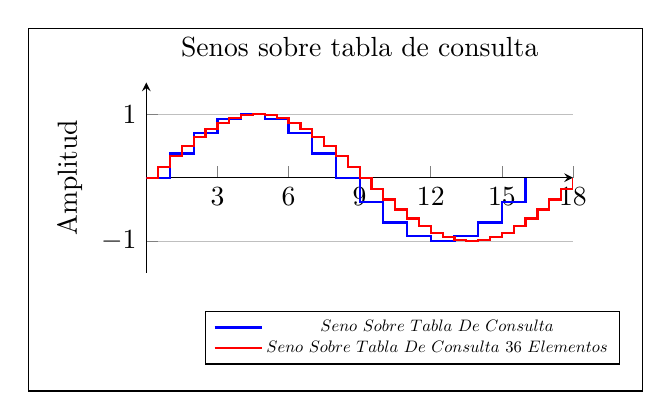
\begin{tikzpicture}
	\draw (-1.5,-1.5) -- (6.3,-1.5) -- (6.3,3.1) -- (-1.5,3.1) -- (-1.5,-1.5);
	\begin{axis}[
		legend style={nodes = {scale=0.6, transform shape}, at={(1.11,-0.2)}},
		legend entries={$Seno\ Sobre\ Tabla\ De\ Consulta$\\$Seno\ Sobre\ Tabla\ De\ Consulta\ 36\ Elementos$\\},
		ymajorgrids=true,
		width=7cm,
		height=4cm,
		x axis line style={-stealth},
		y axis line style={-stealth},
		title={Senos sobre tabla de consulta},
		ymax = 1.5,xmax=18,
		ymin = -1.5, xmin = 0,
		axis lines*=center,
		xtick distance=3,
		ytick={-1,0,1},
		ylabel={Amplitud},
		xlabel near ticks,
		ylabel near ticks]
		\addplot+[blue, thick, no marks, const plot]
		coordinates{
			( 0 , 0.0000 )( 1 , 0.3827 )( 2 , 0.7071 )( 3 , 0.9239 )( 4 , 1.0000 )( 5 , 0.9239 )( 6 , 0.7071 )( 7 , 0.3827 )( 8 , 0.0000 )( 9 , -0.3827 )( 10 , -0.7071 )( 11 , -0.9239 )( 12 , -1.0000 )( 13 , -0.9239 )( 14 , -0.7071 )( 15 , -0.3827)(16, 0)
		};
		\addplot+[red, thick, no marks, const plot]
		coordinates{(0.0 , 0.0000 )( 0.5 , 0.1736 )( 1.0 , 0.3420 )( 1.5 , 0.5000 )( 2.0 , 0.6428 )( 2.5 , 0.7660 )( 3.0 , 0.8660 )( 3.5 , 0.9397 )( 4.0 , 0.9848 )( 4.5 , 1.0000 )( 5.0 , 0.9848 )( 5.5 , 0.9397 )( 6.0 , 0.8660 )( 6.5 , 0.7660 )( 7.0 , 0.6428 )( 7.5 , 0.5000 )( 8.0 , 0.3420 )( 8.5 , 0.1736 )( 9.0 , 0.0000 )( 9.5 , -0.1736 )( 10.0 , -0.3420 )( 10.5 , -0.5000 )( 11.0 , -0.6428 )( 11.5 , -0.7660 )( 12.0 , -0.8660 )( 12.5 , -0.9397 )( 13.0 , -0.9848 )( 13.5 , -1.0000 )( 14.0 , -0.9848 )( 14.5 , -0.9397 )( 15.0 , -0.8660 )( 15.5 , -0.7660 )( 16.0 , -0.6428 )( 16.5 , -0.5000 )( 17.0 , -0.3420 )( 17.5 , -0.1736 )(18, 0.0000)};
	\end{axis}
\end{tikzpicture}\\
Desde la gráfica de estas dos funciones podemos deducir que mientras más elementos tenga nuestras tablas de consulta mayor va a ser la precisión del seno.
Sabiendo el valor de los senos en un punto X podemos llegar a un valor de $D_{c}$ para poder generar una onda cuasi analógica.

\section*{El Principal Problema}
Nuestra placa de desarrollo, la RP2040 no cuenta con un F.P.U. debemos usar nuestro A.L.U. para simular coma flotante desde assembler debemos crear nuestro dato.
\end{document}
